\chapter{Fundamentação Teórica}\label{cap:fundamentacao-teorica}

Este capítulo apresenta a fundamentação teórica, separada em aspectos de saúde e
tecnológicos. As seções de saúde abordam termos como Assistência Domiciliar à
Saúde e suas particularidades, além de explanar, brevemente, sobre a história da
hospitalização no Brasil. A seção \ref{sec:aspectos-tecnologicos} trata das
tecnologias e conceitos tecnológicos utilizados neste trabalho.

\section{Aspectos de Saúde}\label{sec:aspectos-de-saude}

Segundo Inaiá Mello, no livro ``Humanização nos Hospitais do Brasil''
\cite{inaia2008}, uma das primeiras instituições voltadas para o cuidado com a
saúde, foi a fundação da Santa Casa de Misericórdia de Santos, em 1543, cuja
principal atividade era prestar assistência de cunho caritativo a pessoas pobres
e desabrigados. Tal estrutura permanece inalterada até o final do século XIX,
e início do século XX.

Com o Governo Getúlio Vargas, a partir de 1930, ocorre no Brasil o processo de
industrialização, que trouxe crescimento rápido e desordenado às cidades,
principalmente São Paulo e Rio de Janeiro. As transformações econômicas e
sociais resultantes desse processo, a falta de saneamento básico, a pobreza etc
foram motivos para que parte da população reivindicasse mais atenção do Governo
em relação aos cuidados de saúde \cite{carvalho1984}.

Carvalho indica, ainda, que apesar dessa pressão, não existiu uma política de
saúde clara por parte das autoridades. Muitas vezes, algumas ações se voltavam
para a criação de condições sanitárias mínimas, que se mostravam limitadas
frente às reais necessidades da população. Dessa forma, as décadas subsequentes
não foram significativas no tocante a uma ampliação dos serviços de saúde
oferecidos à população.

Conforme análise de Inaiá Mello, ainda nos anos 1970, surgem tentativas de
universalizar o acesso à assistência à saúde. Alguns Programas e Sistemas foram
iniciados, sendo válido citar, (i) Sistema Único e Descentralizado de Saúde, o
SUDS e (ii) o Sistema Único de Saúde, o SUS. Entretanto, em virtude da vigência
da ditadura militar, implantada em 1964, que levou o país a vivenciar um estado
de exceção, tais propostas não conseguiram se concretizar. Assim, somente no
período da redemocratização, ocorrida em meados dos anos 1980, é que o SUS foi
criado oficialmente pela Constituição Federal de 1988, Lei 8080/90
\footnote{Acessível em
\url{http://www.planalto.gov.br/ccivil_03/leis/L8080.htm}}, com o objetivo de
garantir à população Brasileira, o acesso universal às ações e serviços de
saúde.

Paralelo à criação do Sistema Único de Saúde (SUS), ocorreu o avanço tecnológico
que alcançou a prática médica, aperfeiçoando, com isso a infraestrutura
hospitalar. Dessa forma, os hospitais deixaram de ser espaços para abrigarem
pobres desamparados e passaram a proporcionar tratamentos mais elaborados. O
hospital passa a oferecer  procedimentos cirúrgicos, atendimentos de urgência,
internações, tornando a instituição dispendiosa. Os estudiosos começam a
identificar a possibilidade de tratamentos e cuidados com a  saúde que não
estejam, necessariamente, vinculados ao ambiente hospitalar.

Como consequência, surgiram diversas mudanças no atendimento, onde a Assistência
Domiciliar à Saúde (ADS) se tornou uma modalidade disponível.

\subsection{Assistência Domiciliar à Saúde}
\label{subsec:assistencia-domiciliar-a-saude}

A Assistência Domiciliar à Saúde (ADS) divide-se basicamente em grupos de
enfermagem e fisioterapia - nas modalidades mais básicas - até um atendimento
multiprofissional, possibilitando um apoio ao paciente como um todo. A ADS pode
ser provida tanto pelo setor privado quanto pelo setor público
\cite{amaral2001assistencia}.

Os primeiros registros da ADS no Brasil surgem em 1967, na cidade de São
Paulo, no Hospital do Servidor Público. O principal objetivo dessa abordagem
era a liberação de leitos no hospital, levando para o domicílio procedimentos
básicos, de baixa complexidade clínica.

Já na década de 90, segundo Tavolari, houve um aumento considerável na
quantidade de empresas privadas provendo o serviço de ADS, apenas 5 empresas
prestavam esse tipo de  serviço, já em 1999, esse número subiu para mais de 180
\cite{tavolari2000desenvolvimento}.

Amaral et al define a ADS como uma sequência de serviços residuais a serem
oferecidos, depois que o indivíduo já recebeu atendimento primário e prévios,
ou seja, aquele que já recebeu atendimento primário com consequente diagnóstico
e tratamento.

Amaral e Tavolari lembram, ainda, que o atendimento domiciliar pode acelerar a
recuperação do  paciente e promover a redução de custos hospitalares, além de
ser uma solução mais  humanista para os portadores de doenças crônicas ou de
longa duração, frente à  hospitalização. Dessa forma, a assistência domiciliar à
saúde, tem como objetivos principais: (1) humanização no atendimento; (2) maior
rapidez na recuperação do paciente, devido à proximidade com os seus familiares;
(3) diminuição do risco de infecção hospitalar; (4) Otimização de leitos
hospitalares para pacientes que deles necessitem; e (5) Redução do custo/dia da
internação.

\subsubsection{Envolvidos}\label{subsubsec:envolvidos}

Para o entendimento geral da modalidade ADS, faz-se necessário separar e
explicar a atuação de cada um dos envolvidos. O paciente, componente principal
é aquele que sofre algum problema físico ou mental. A família é responsável
por prover um ambiente propício à melhora do paciente.

Outra figura importante na atenção ao paciente é a equipe multiprofissional -
composta de médicos, enfermeiros, psicólogos, terapeutas, assistentes sociais,
farmacêuticos, cuidadores e outros - visando propiciar, através da integração
das diversas áreas de conhecimentos, a melhoria efetiva do paciente.

O cuidador, muitas vezes, é um familiar, alguém próximo à família ou alguém
contratado. Seu papel principal é cuidar do paciente, ajudando nas tarefas
diárias, como alimentação, lazer, socialização, limpeza do paciente, entre
outros \cite{amaral2001assistencia}.

%Embora as pesquisas indiquem que o tratamento domiciliar ajuda na recuperação do
%paciente, devido sua presença no seio familiar, também sabemos das dificuldades
%que os cuidadores enfrentam. exemplo quando são familiares, que muitas vezes, 
%negam a dar atenção, ou desempenhar determinadas funções.

\subsubsection{Terminologia}\label{subsubsec:terminologia}

Apesar de não haver uma definição formal, a Assistência Domiciliar à Saúde pode
ser separada em três modalidades, diferenciadas, principalmente, pelo grau de 
atenção dispensada ao paciente. 

É defendido por Tavolari, Fernandes e Medina, que o termo Assistência Domiciliar
à Saúde é genérico e referente a todo e qualquer procedimento de saúde realizado
em domicílio, não importando o grau de complexidade. Já o termo Internação
Domiciliar é aplicado quando, dos procedimentos realizados, o cuidado intensivo
e multiprofissional é perceptível, caracterizando-se ainda, pelo transporte de
parte da estrutura hospitalar para o domicílio do paciente. O paciente, nesse
caso, é categorizado com complexidade alta ou moderada.
Já no Atendimento Domiciliar, o paciente encontra-se num estado de menor 
complexidade médica, e a atenção a ele dispensada, pode ou não ser realizada por
uma equipe multiprofissional \cite{tavolari2000desenvolvimento}.

  \begin{figure}[H]
    \begin{center}  
    \caption{(a) Representação gráfica das categorias defendida por Tavolari,
    Fernandes e Medina; (b) Representação gráfica das categorias defendida
    por Giacomozzi.}
      \begin{subfigure}[b]{.45\textwidth}
        % \resizebox{6cm}{5cm}{
         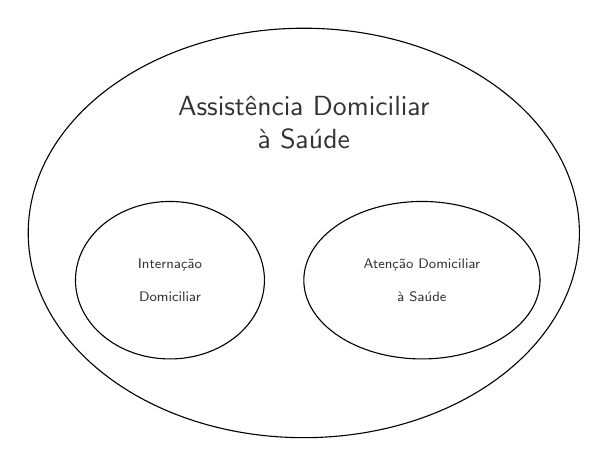
\begin{tikzpicture}[font=\sffamily]
         \begin{scope}[shift={(0cm,0cm)}, fill opacity=0.8]
             \draw (0,0) ellipse (3.5cm and 2.6cm);
             \draw (-1.7,-0.6) ellipse (1.2cm and 1cm);
             \draw (1.5,-0.6) ellipse (1.5cm and 1cm);

             \node at (0,1.4) [align=center]{Assistência Domiciliar\\ à Saúde};
             \node at (-1.7,-0.6) [align=center]{\tiny Internação\\ \tiny Domiciliar};
             \node at (1.5,-0.6)[align=center]{\tiny Atenção Domiciliar\\ \tiny à Saúde};
             \end{scope}
         \end{tikzpicture} 
         % } % close resizebox
        \caption{}
        \label{fig:ads-categoria-tavoloari}
      \end{subfigure}
      ~
      \begin{subfigure}[b]{.45\textwidth}
        % \resizebox{6cm}{5cm}{
        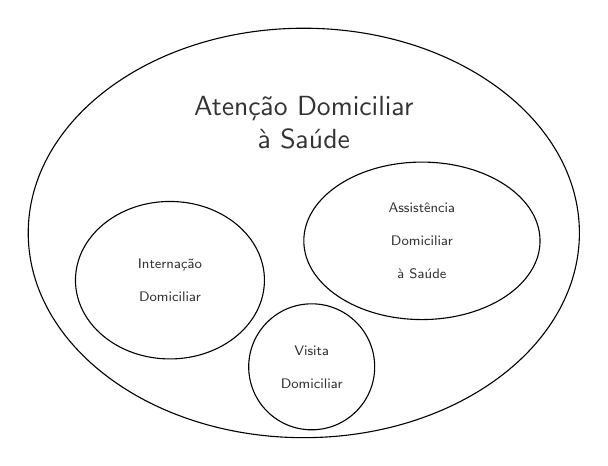
\begin{tikzpicture}[font=\sffamily]
        \begin{scope}[shift={(0cm,0cm)}, fill opacity=0.8]
            \draw (0,0) ellipse (3.5cm and 2.6cm); % atencao domiciliar
            \draw (-1.7,-0.6) ellipse (1.2cm and 1cm); % internacao domiciliar
            \draw (1.5,-0.1) ellipse (1.5cm and 1cm); % assistencia domiciliar
            \draw (0.1, -1.7) circle (0.8cm); % visita domiciliar

            \node at (0,1.4) [align=center]{Atenção Domiciliar\\ à Saúde};
            \node at (-1.7,-0.6) [align=center]{\tiny Internação\\ \tiny Domiciliar};
            \node at (1.5,-0.1)[align=center]{\tiny Assistência\\ \tiny Domiciliar\\ \tiny à Saúde};
            \node at (0.1,-1.7)[align=center]{\tiny Visita\\ \tiny Domiciliar};
            \end{scope}
        \end{tikzpicture}
        % } % close resizebox
        \caption{}
        \label{fig:ads-categoria-giacamozzi}
      \end{subfigure}
      \par
      Fonte: Próprio autor.
    \end{center}
  \end{figure}

Giacomozzi faz uma inversão das categorias propostas por Tavolari et al. e 
define Atenção Domiciliar à Saúde, como um termo mais genérico, englobando
o atendimento, a visita e as internações domiciliares \cite{giacomozzi2006pratica}.
Segundo a autora, a atenção domiciliar é ``um
componente do \textit{continuum} dos cuidados à saúde, pois os serviços de
saúde são oferecidos ao indivíduos e sua família [...] minimizando os efeitos
das incapacidades ou doenças, incluindo aquelas sem perspectiva de cura.''
Já o termo Assistência Domiciliar à Saúde, é formado por atividades de cunho 
ambulatorial, adicionando a essa categorização a modalidade Visita Domiciliar,
voltada para verificar a realidade do paciente, além de realizar ações educativas.  

A despeito da diversidade de categorização apresentada pelos autores, ao nosso
trabalho interessa tanto aqueles pacientes que inspiram maiores cuidados,
correndo, inclusive, risco de vida, quanto aqueles que demandam menos
preocupações.

% \subsection{Urgência e Emergência}\label{subsec:urgencia-emergencia}
% \lipsum[1]

% \subsection{Atenção domiciliar}\label{subsec:atencao-domiciliar}
% \lipsum[1]

\section{Aspectos Tecnológicos}\label{sec:aspectos-tecnologicos}

Este trabalho foi amparado em tecnologias bem conhecidas, permitindo assim, 
que os objetivos fossem alcançados.

\subsection{Sistemas Embarcados}\label{subsec:sistemas-embarcados}

Sistemas Embarcados estão inseridos em nossos cotidianos. Aparelhos como
\smartphones[], \tablets[] - com alto poder de processamento,
produtos comumente encontrados em nossas casas, a exemplo do forno de 
micro-ondas, geladeiras e máquinas de lavar roupas, até computadores de bordo e
controle de freios ABS (\textit{Anti-lock Breaking System})\footnote{ABS:
Tecnologia  de freio considerada segura pois seu funcionamento impede que, em
uma brecada brusca, as rodas  deslizem, tornando difícil controlar o veículo} em
nossos carros, contêm sistemas embarcados. Essa diversidade de aplicações
explicita a importância dessa área.

Nos exemplos citados anteriormente, temos uma classificação quanto à sua
funcionalidade, porém, sua definição não é simples, nem muito menos taxativa,
uma vez que possuem uma grande complexidade em sua composição. Dessa forma,
podemos definir, informalmente, sistemas embarcados como qualquer
dispositivo/equipamento que disponha de um sistema programável e que seu
objetivo não seja o de um computador de propósito geral\footnote{Computador de
propósito geral é aquele em que é possível executar as mais diversas tarefas,
tais como, navegar na Internet, escrever documentos, executar jogos etc, ou
seja, não há uma função específica a ser realizada. Pelo exposto, percebe-se a
complexidade da sua definição, uma vez que, muitos desses sistemas embarcados
desempenham funções que antes cabiam apenas ao computador de propósito geral.}
\cite{wolf2012computers}.

Marwedel define: ``Sistemas Embarcados são sistemas de processamento de
informações incorporados à produtos.'', adicionado à esta definição, lista 5
características que sistemas embarcados devem levar em consideração: 

\begin{itemize}
  \item Segurança - ou seja, os dados confidenciais transmitidos ou recebidos pelo
  equipamento devem permanecer confidenciais e a comunicação deve ser autêntica;
  \item Seguro - característica indicativa de que o sistema não causará nenhum dano;
  \item Disponibilidade - sistema disponível para executar as funções para as quais
  foi programado; 
  \item Confiabilidade - probabilidade que o sistema tem de que não
  falhará em sua execução; e
  \item Manutenabilidade, característica  que se o sistema vir a falhar, deverá 
  ser concertado em uma determinada janela de tempo.
\end{itemize}

Além disso, propriedades como, sensores coletando informações do ambiente
físico e atuadores controlando o ambiente no qual estão inseridos também
caracterizam um sistema embarcado \cite{marwedel2010embedded}.

\subsubsection{Arquitetura}\label{subsubsec:arquitetura}

A literatura divide o sistema embarcado em duas áreas, o \hardware[] e o 
\software. O primeiro é composto pelas partes físicas do sistema, 
tal como o processador, memória, interfaces de entrada e saída etc. O segundo é
composto pelos componentes lógicos do sistema, ou seja, os programas que 
irão executar as funções previamente definidas do sistema embarcado.

No processo de \design[] do sistema embarcado considera-se, dentro dos
requisitos de \hardware, quais dos processadores disponíveis no mercado atende
melhor a necessidade do projeto, além da quantidade de memória disponível para o
\software[] utilizar. Outro ponto a ser determinado são as interfaces de entrada
e saída - responsáveis por receber dados para processar e apresentar os dados
processados respectivamente. Em paralelo, os requisitos de \software[] são
alinhados para que o \hardware[] seja melhor aproveitado
\cite{wolf2012computers}.

A depender da finalidade do produto, esses requisitos diferem bastante. Por
exemplo, o sistema embarcado responsável por controlar uma máquina de lavar é
simples (em termos de funcionalidade, processamento, consumo de energia etc),
uma vez que aplica um componente microcontrolador de baixo poder de
processamento (tal qual um microprocessador PIC de 16 bits) e um circuito
auxiliar para atender as especificações de entrada e saída do sistema, assim
como uma possível comunicação com outros sistemas.

Já o sistema embarcado em um \smartphone[] realiza diversas funções, tem um
alto nível de processamento de dados e consome muita energia. Para atender a
estes requisitos, a equipe responsável pelo \design[] utiliza vários
processadores de alto poder computacional (tal qual processadores ARM), como
interface de entrada e saída uma tela sensível ao toque e faz uso, ainda, de
diversos sensores para ajudar na usabilidade do dispositivo.

Semelhante aos \smartphones, o sistema embarcado utilizado neste trabalho, o
Set-Top Box (STB), processa grande quantidade de dados, porém não funciona a
bateria. Apesar dessa diferença o \hardware[] utilizado é bastante semelhante.

\subsection{Computação ubíqua e pervasiva}\label{subsec:computacao}

A convergência das diversas tecnologias pode ser observado no nosso dia-a-dia
através de: informações constantes que recebemos nos dispositivos móveis, nos
meios de comunicação, do monitoramento em tempo real do tráfego nas cidades de
grande porte, dos relógios com tecnologia embarcada (\textit{smartwatches}), das
vestimentas inteligentes etc.

Percebemos, também, o distanciamento ou o desaparecimento da figura ``computador
pessoal (PC)'' em nosso cotidiano. A tecnologia está difundida ao ponto do termo 
``era pós pc'' ser encontrado em diversos estudos \cite{bonilla2011inclusao, 
chen2011pospc, press1999personal} nas áreas de sistemas embarcados e 
tecnologias móveis.

À essa tecnologia ``em todo lugar'' e o distanciamento do usuário com o 
computador pessoal deu-se o nome de computação ubíqua. Mark Weiser, considerado 
o pai desse termo, profetizou que encontraríamos tecnologia nos diversos objetos
do nosso cotidiano, tais como etiquetas de roupas e alimentos, cadeiras, 
geladeiras, lixeiras, interruptores de luzes etc \cite{weiser1991computer}.

Através de sensores e meios de comunicação, esses objetos ganham novas funções.
A patente de Yang registra uma lixeira inteligente que abre sua tampa de acordo
com a proximidade do usuário \cite{yang2005trash}. Já a pesquisa de Wang
demonstra a utilização de sensores em uma geladeira. A partir de um sistema de
gerenciamento da geladeira é possível ter informações das comidas e recomendar
receitas para o usuário de acordo com os alimentos disponíveis, além de 
verificar quais itens estão próximos do final da validade ou faltantes e gerar 
uma lista de compras personalizada \cite{hou2013}.

% Os dispositivos \smartphones, \tablets, relógios inteligentes e até mesmo roupas
% inteligentes são realidades para muitos. Esses dispositivos permitem que o 
% indivíduo que os carrega, tenha um poder computacional que o permita utilizar 
% serviços que um computador oferece, independentemente da sua localização 
% \cite{de2003computaccao}.

Muitas vezes, a tecnologia inserida nesses objetos é invisível para o usuário 
final e essa transparência era defendida por Weiser para apresentar um outro 
termo, a ``computação pervasiva''. Weiser a define informalmente: ``(...) criar 
um computador tão embarcado, tão natural que o usaríamos sem nem pensar sobre 
ele'', além disso computação pervasiva está relacionada à capacidade de 
dispositivos serem embarcados no mundo físico, obtendo informações do meio para 
auxiliar na computação, integrando assim, o ambiente físico e o mundo virtual
\cite{bolsoni2009computaccao, de2003computaccao}.

Segundo Hansmann, a computação pervasiva tem 4 princípios fundamentais,
detalhados a seguir:

\begin{description}
  \item [Descentralização] os diversos dispositivos cooperam entre si e realizam
  pequenas tarefas e funções, contribuindo para o estabelecimento de uma 
  dinâmica rede de comunicação;
  \item [Diversificação]  
  \item [Conectividade] os dispositivos devem interagir de maneira transparente
  e àqueles que são móveis, devem mudar entre redes heterogêneas sem o 
  auxílio de um usuário; e
  \item [Simplicidade] as funções desempenhadas pelos dispositivos devem ser
  simples e de fácil execução, para aqueles que detém alguma forma de interação
  com o usuário, devem ser de fácil utilização.
\end{description}

No que concerne à assistência domiciliar à saúde, as pesquisas nas áreas de
computação ubíqua e computação pervasiva são as mais diversas.

O domicílio é um ambiente propício para exemplificar os conceitos de computação
pervasiva e ubíqua pois nele são utilizados dispositivos capazes de 

Pesquisas realizadas demonstram a utilização de sensores , como por exemplo o estudo de Norbet, em que sensores magnéticos posicionados em portas e


Podemos exemplificar esses conceitos no ambiente domiciliar e nos casos de 
assistência domiciliar levando em consideração os diversos dispositivos que 
os pacientes carregam consigo, com os equipamentos eletrônicos

\subsection{Aplicações Sensíveis ao Contexto}\label{subsec:contexto}




























